\documentclass{standalone}

\usepackage{tikz}
    \usetikzlibrary{arrows.meta}
    % \usetikzlibrary{calc}
    
\begin{document}
\begin{tikzpicture}
    % \draw[help lines] (-1,-1) grid (11,5);
    \node at (2,2) {
\includegraphics[width=4.25cm]{pictures/2fip_F1.png}};
    \node at (9,2) {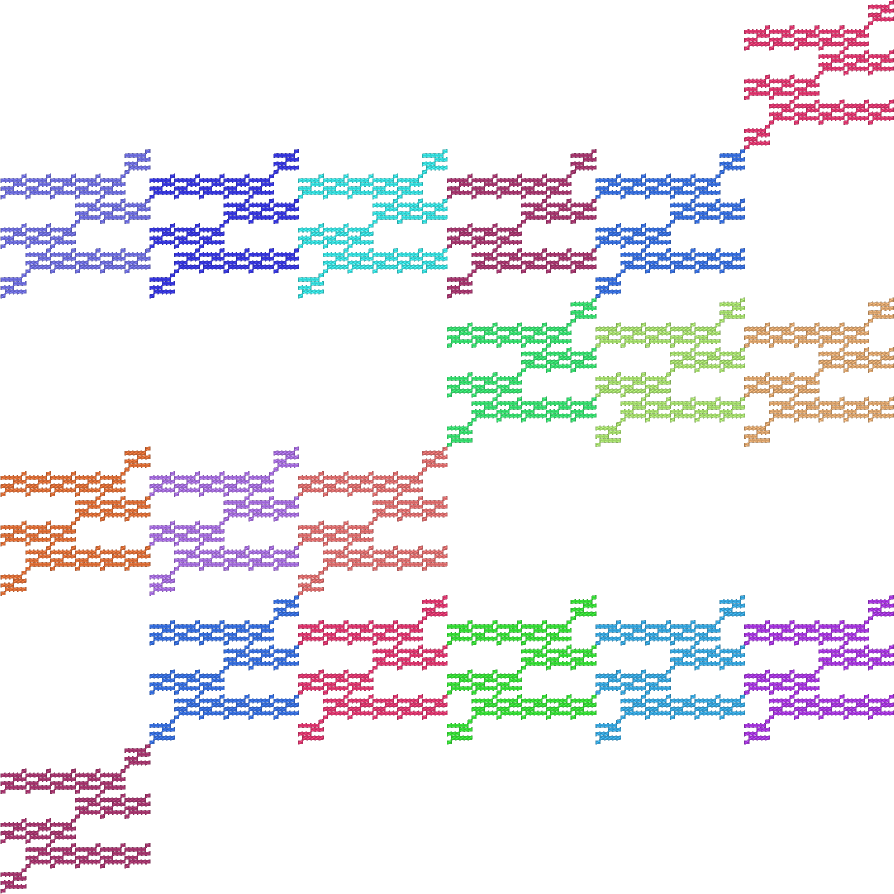
\includegraphics[width=4cm]{pictures/2fip_F.png}};
    \path[->,>={Latex[length=3mm]}, line width=0.5mm]
        (-0.5,-0.5) edge (0,0)
        (4.5,4.5) edge (4,4)
        (6.5,-0.5) edge (7,0)
        (11.5,4.5) edge (11,4)
        (-0.7,1.33) edge[red] (0,1.33)
        (4.7,1.33) edge[red] (4,1.33)
        (6.3,1.33) edge[red] (7,1.33)
        (11.7,1.33) edge[red] (11,1.33)
        (-0.7,2.66) edge[blue] (0,2.66)
        (4.7,2.66) edge[blue] (4,2.66)
        (6.3,2.66) edge[blue] (7,2.66)
        (11.7,2.66) edge[blue] (11,2.66);
\end{tikzpicture}
\end{document}